\section{Архитектура системы планирования производства}
\indent Система планирования производства представляет из себя набор программных модулей, взаимодействующих согласно схеме (рисунок \ref{fig:archSPP}).

\begin{figure}[ht]
	\centering
	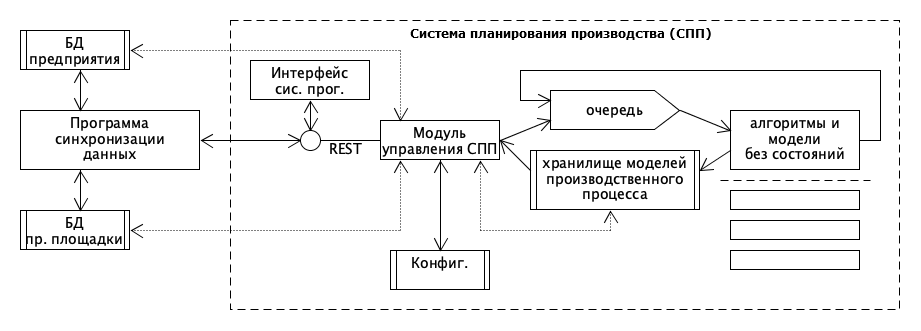
\includegraphics[width=\linewidth]{pics/archSPP.png}
	\caption{Схема системы планирования производства \cite{niorkpz}}
	\label{fig:archSPP}
\end{figure}

\indent В силу необходимости в планировании различных вариантов работы производства, каждый из которых отличается конфигурацией смен либо количеством доступных ресурсов, система производит запуск множества параллельных расчетов, по результатам которых впоследствии сотрудник сможет выбрать оптимальный.
За запуск и синхронизацию отвечает ``Модуль управления СПП'' (рисунок \ref{fig:archSPP}), который создает очередь расчетов на запуск.
Затем пул потоков (автоматическое средство для задач, которые требуют временных запусков потоков) извлекает их в порядке очереди и запускает работу подсистемы имитационного моделирования в отдельном потоке (``Алгоритмы и модели без состояний'', рисунок \ref{fig:archSPP}).
После окончания работы полученный результат передается обратно в модуль управления для возврата пользователю посредством RESTful API (веб-служба, построенная с учетом архитектурного стиля REST~--~ стиль взаимодействия компонентов распределённого приложения в сети).
Пользователь, зная с какими параметрами запускался полученный расчет, может поменять конфигурацию и отправить его на повторное вычисление.
Конфигурация измененного расчета будет сохранена в базе данных предприятия и приведет к запуску всего цикла с начала.